\documentclass[11pt,a4paper]{article}

\usepackage[spanish]{babel}
\usepackage[utf8]{inputenc}
\usepackage[T1]{fontenc}
\usepackage{amsmath,amssymb}
\usepackage{geometry}
\usepackage{enumitem}
\usepackage{graphicx}
\usepackage{float}
\geometry{margin=2.5cm}

\begin{document}

\begin{titlepage}
\centering
{\Large \textbf{UNIVERSIDAD TECNOLÓGICA DE PEREIRA}}\\[0.8cm]
{\large INGENIERÍA DE SISTEMAS Y COMPUTACIÓN}\\[0.5cm]
{\large HPC: HIGH PERFORMANCE COMPUTING}\\[2.0cm]
{\LARGE \textbf{Análisis del Algoritmo de Jacobi Iterativo para la Ecuación de Poisson 1D}}\\[0.8cm]

\begin{flushleft}
\textbf{Autor:} Jorge Luis López Grajales\\[0.4cm]
\textbf{Asignatura:} HPC: High Performance Computing\\[0.4cm]
\textbf{Docente:} Ramiro Andrés Barrios Valencia\\[0.4cm]
\textbf{Fecha:} \today
\end{flushleft}
\vfill
{\large Pereira -- Colombia}
\end{titlepage}

\section{Análisis del Algoritmo de Jacobi Iterativo}

El problema consiste en resolver la ecuación de Poisson en una dimensión:
\[
-u'' = f(x)
\]
en un dominio $[a,b]$ con condiciones de frontera de Dirichlet.

\subsection{Formulación matemática y discretización}

Para aproximar la solución, dividimos el dominio en $N$ puntos con un espaciado constante $h$.  
Aplicando diferencias finitas centradas de segundo orden, la ecuación diferencial se transforma en el sistema:
\[
\frac{-u_{i-1} + 2u_i - u_{i+1}}{h^2} = f(x_i).
\]
Esto genera un sistema lineal $Au=b$, donde $A$ es una matriz tridiagonal.

\subsection{Lógica de la iteración de Jacobi}

El método de Jacobi descompone la matriz $A$ en $D$ (diagonal) y $(L+U)$ (triangulares).  
La actualización de cada nodo para la iteración $k+1$ es:
\[
u_i^{(k+1)} = \frac{1}{2}\left(u_{i-1}^{(k)} + u_{i+1}^{(k)} + h^2 f_i\right).
\]

\textbf{Nota clave:} La independencia de los cálculos en cada nodo $i$ (solo dependen de valores de la iteración previa $k$) convierte a Jacobi en un algoritmo naturalmente paralelo (\emph{embarrassingly parallel}).

\section{Opciones de concurrencia y optimización}

El análisis de implementaciones paralelas y optimizaciones de sistema revela diferencias críticas en eficiencia.

\subsection{Threads (hilos) vs. Fork (procesos)}

\begin{itemize}[leftmargin=1.2cm]
    \item \textbf{Threads:} Utilizan un espacio de memoria compartido. Son ligeros en creación y permiten comunicación inmediata para acceder a los vectores de la malla.
    \item \textbf{Fork:} Crea procesos independientes con su propio espacio de direccionamiento. Aunque existe \emph{copy-on-write}, la sincronización de fronteras de subdominios en cada iteración genera latencia significativa.
\end{itemize}

\subsection{Optimización de memoria}

\begin{itemize}[leftmargin=1.2cm]
    \item \textbf{Gestión del mallado:} Jacobi requiere dos vectores ($u_{old}$ y $u_{new}$).
    \item En hilos, ambos residen en memoria global accesible por todos.
    \item En procesos, se requiere memoria compartida explícita (por ejemplo, \texttt{mmap} o \texttt{shmget}), lo que añade complejidad y sobrecosto.
\end{itemize}

\subsection{Optimización de CPU}

\begin{itemize}[leftmargin=1.2cm]
    \item \textbf{Compilador:} Banderas como \texttt{-Ofast} habilitan vectorización (SIMD) y desenrollado de bucles.
    \item En problemas pequeños ($K<11$), la versión secuencial optimizada puede ser más eficiente que la paralela por ausencia de sincronización.
    \item \textbf{Complejidad:} El costo total crece como $O(n_k^3)$.
    \item Las optimizaciones deben equilibrar reducción del tiempo por iteración (paralelismo) y reducción del número de iteraciones (Gauss-Seidel, SOR).
\end{itemize}

\section{Análisis de resultados de desempeño}

Basado en las gráficas de \emph{speedup} y tiempo obtenidas en los barridos de $K$, se observan las siguientes causas:

\subsection*{A. Sobrecosto de gestión (\emph{overhead})}
Para valores bajos de malla ($K\leq 9$), el \emph{speedup} es menor que 1.

\textbf{Causa:} El tiempo del kernel del SO en crear contexto de hilos o clonar procesos es mayor que el tiempo de cómputo de la malla. En este rango, la versión secuencial optimizada domina.

\subsection*{B. Relación cómputo/comunicación}
El \emph{speedup} de hilos supera 2.0 a partir de $K=12$.

\textbf{Causa:} Al crecer la malla, la carga computacional por iteración aumenta y la penalización de la barrera de sincronización se vuelve relativamente pequeña.

\subsection*{C. Eficiencia de la arquitectura de memoria}
Los hilos superan consistentemente a los procesos en escalabilidad.

\textbf{Causa:} El aislamiento de memoria de \emph{fork} penaliza el rendimiento. Los procesos introducen más contención en planificador y bus de datos, reflejada en picos de inestabilidad temporal.

\subsection*{D. Impacto de la tolerancia}
En barridos de tolerancia, el \emph{speedup} se mantiene casi constante al aumentar la precisión.

\textbf{Causa:} Una tolerancia más estricta (por ejemplo, $10^{-6}$) incrementa iteraciones, pero no la carga por iteración. La proporción cómputo/sincronización se mantiene.

\subsection{Gráficas de desempeño}

\begin{figure}[H]
    \centering
    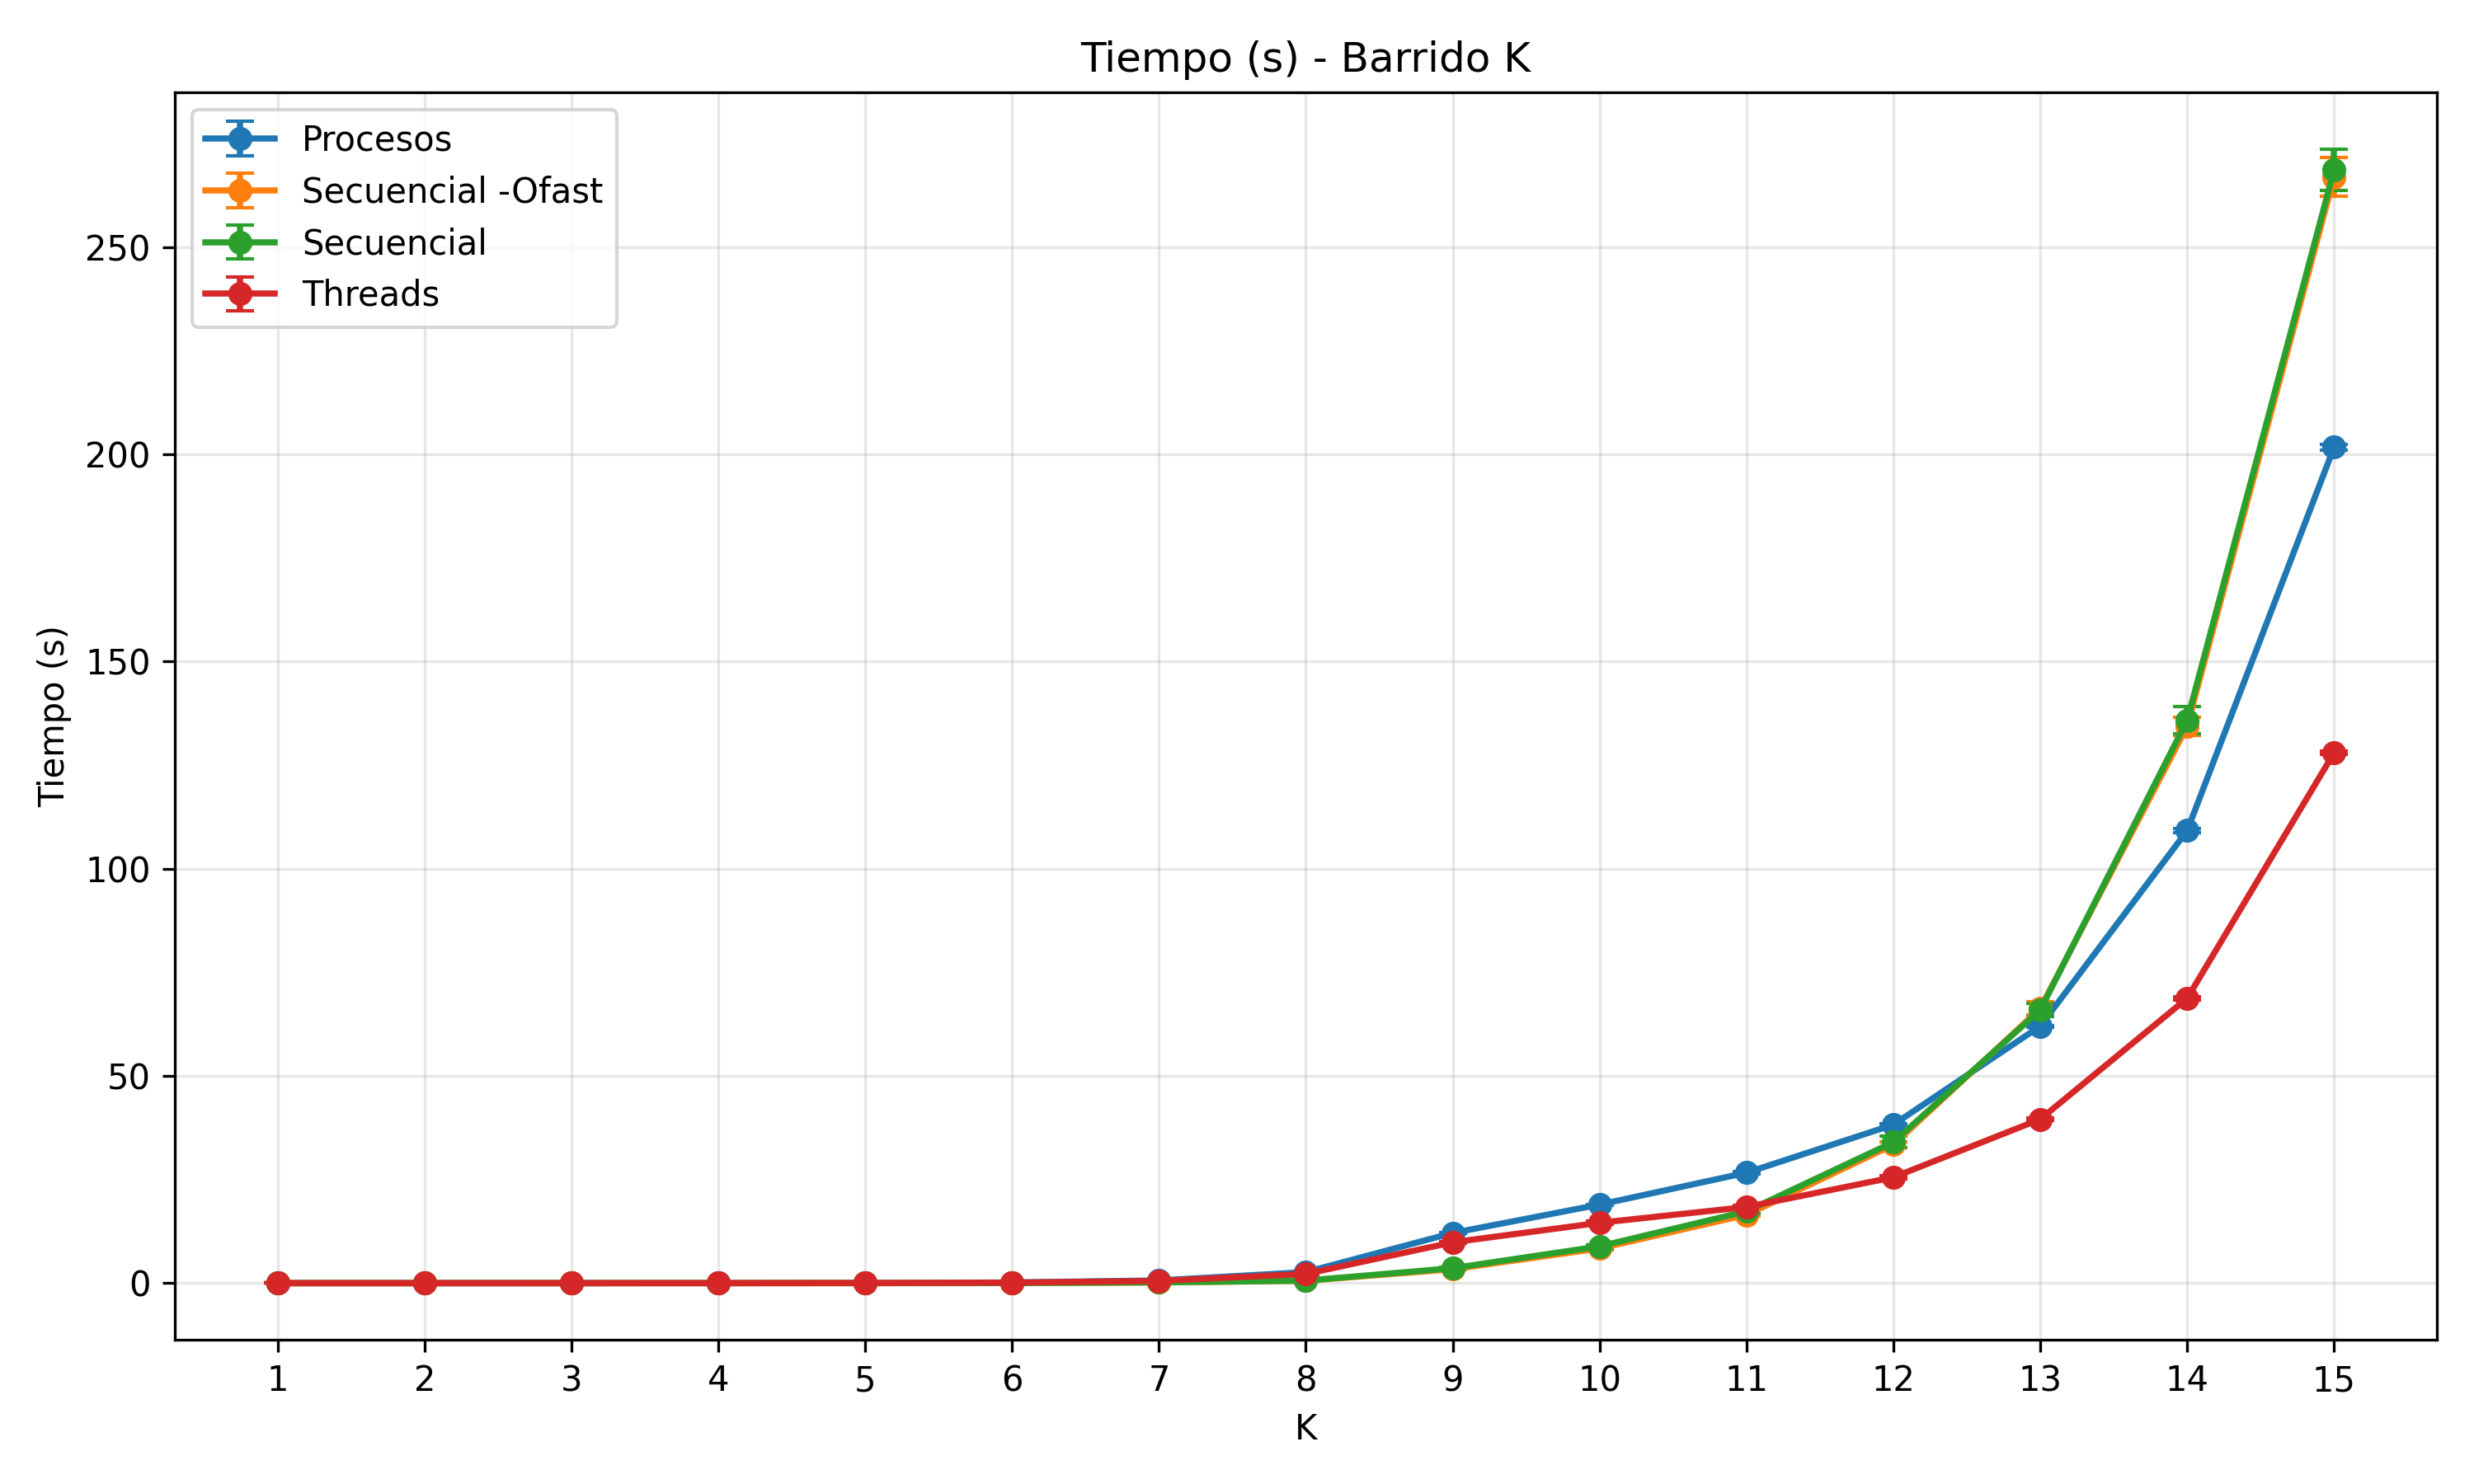
\includegraphics[width=0.85\textwidth]{plots/k_sweep_time_comparison.png}
    \caption{Comparación de tiempos para barrido en $K$.}
\end{figure}

\begin{figure}[H]
    \centering
    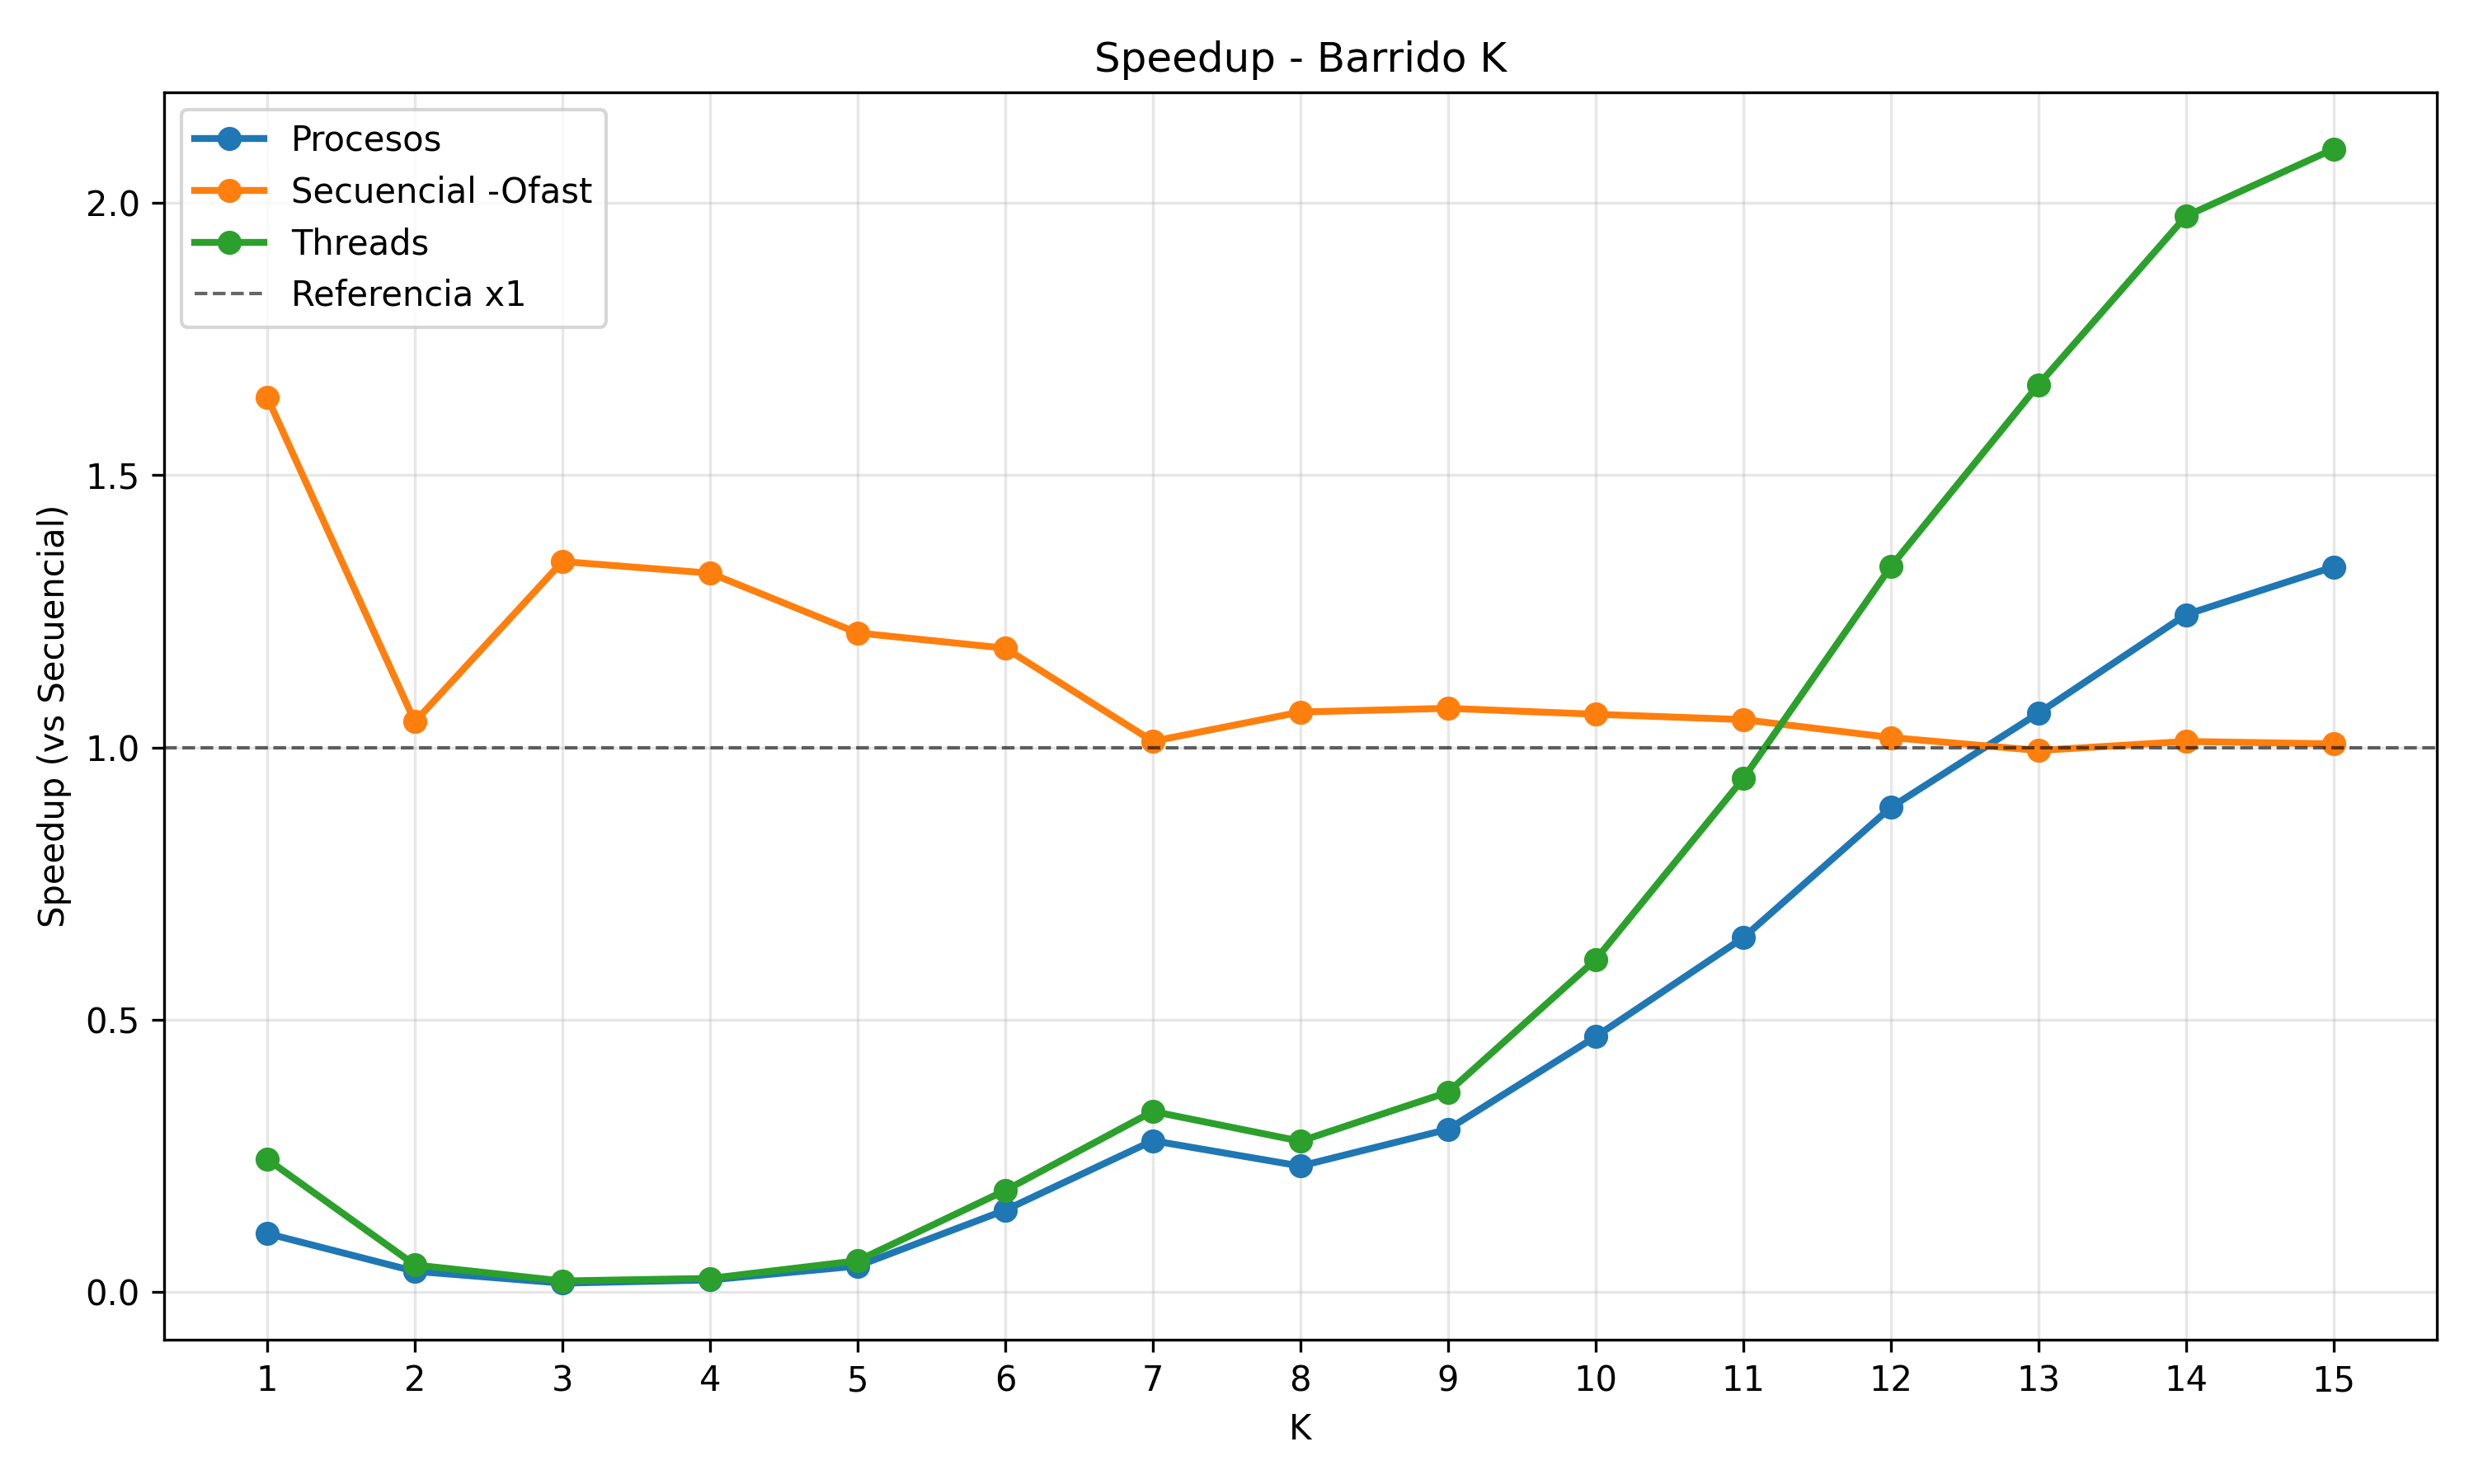
\includegraphics[width=0.85\textwidth]{plots/k_sweep_speedup.png}
    \caption{Speedup (base secuencial) para barrido en $K$.}
\end{figure}

\begin{figure}[H]
    \centering
    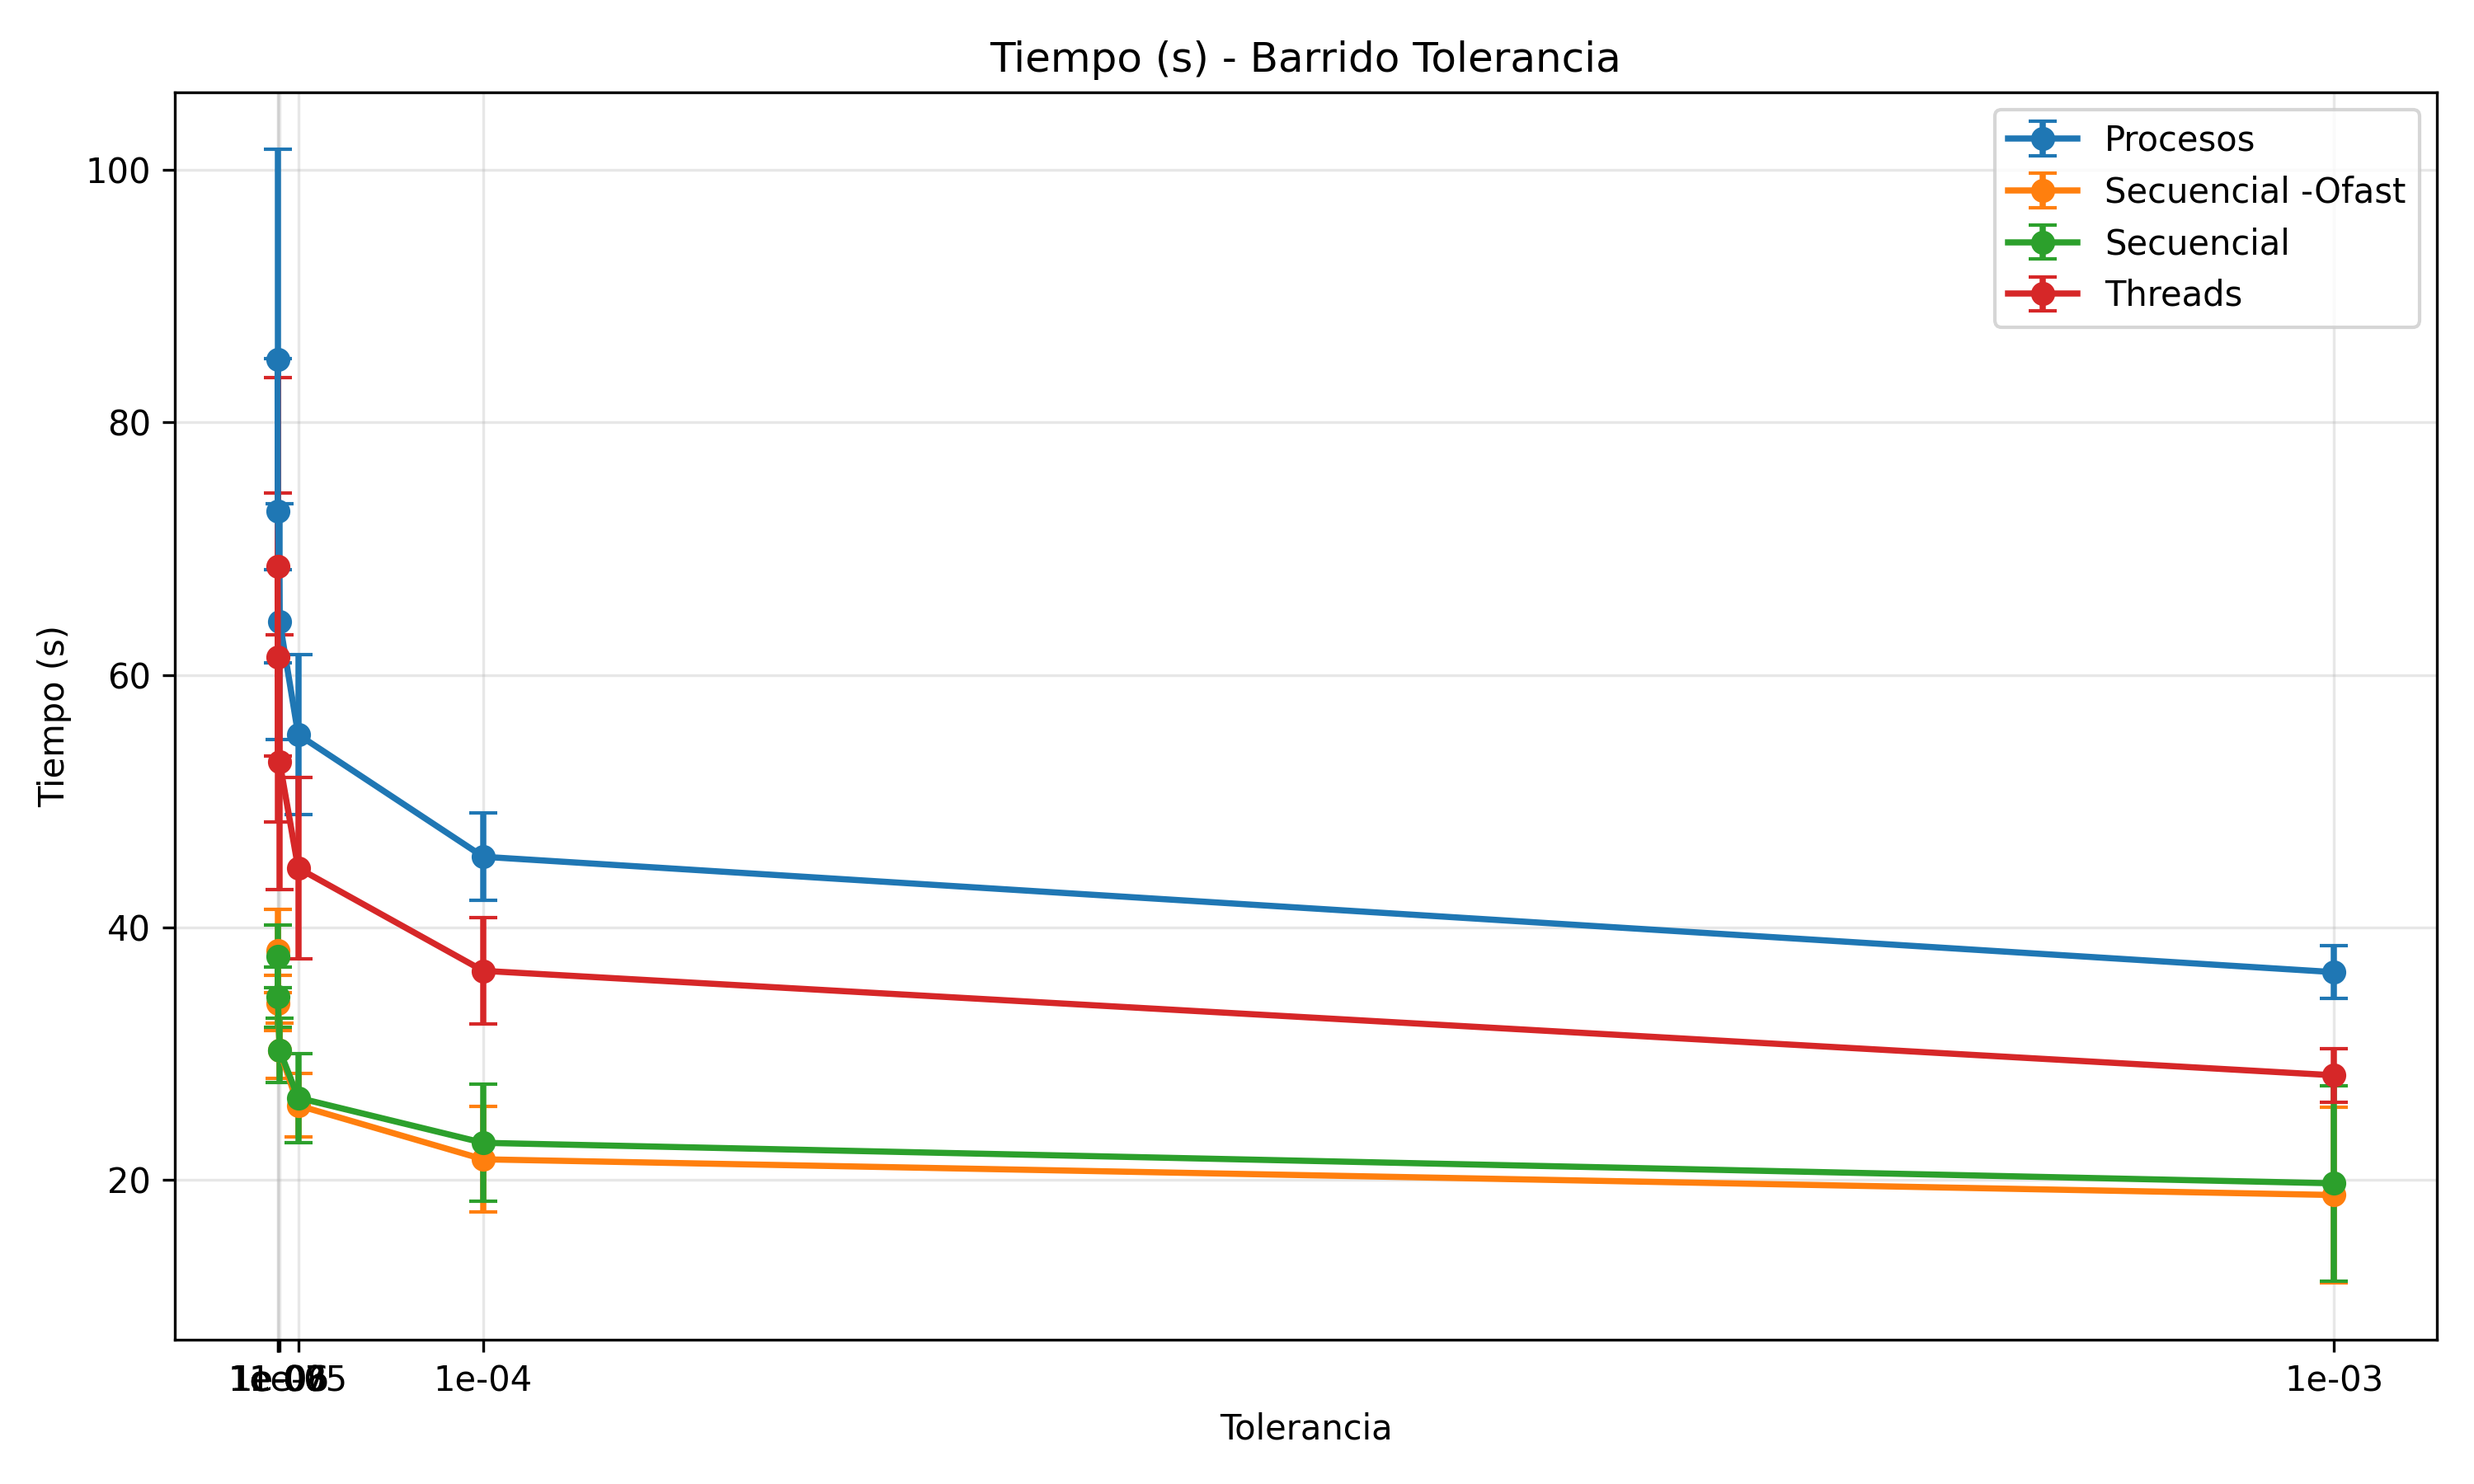
\includegraphics[width=0.85\textwidth]{plots/tol_sweep_time_comparison.png}
    \caption{Comparación de tiempos para barrido de tolerancia.}
\end{figure}

\begin{figure}[H]
    \centering
    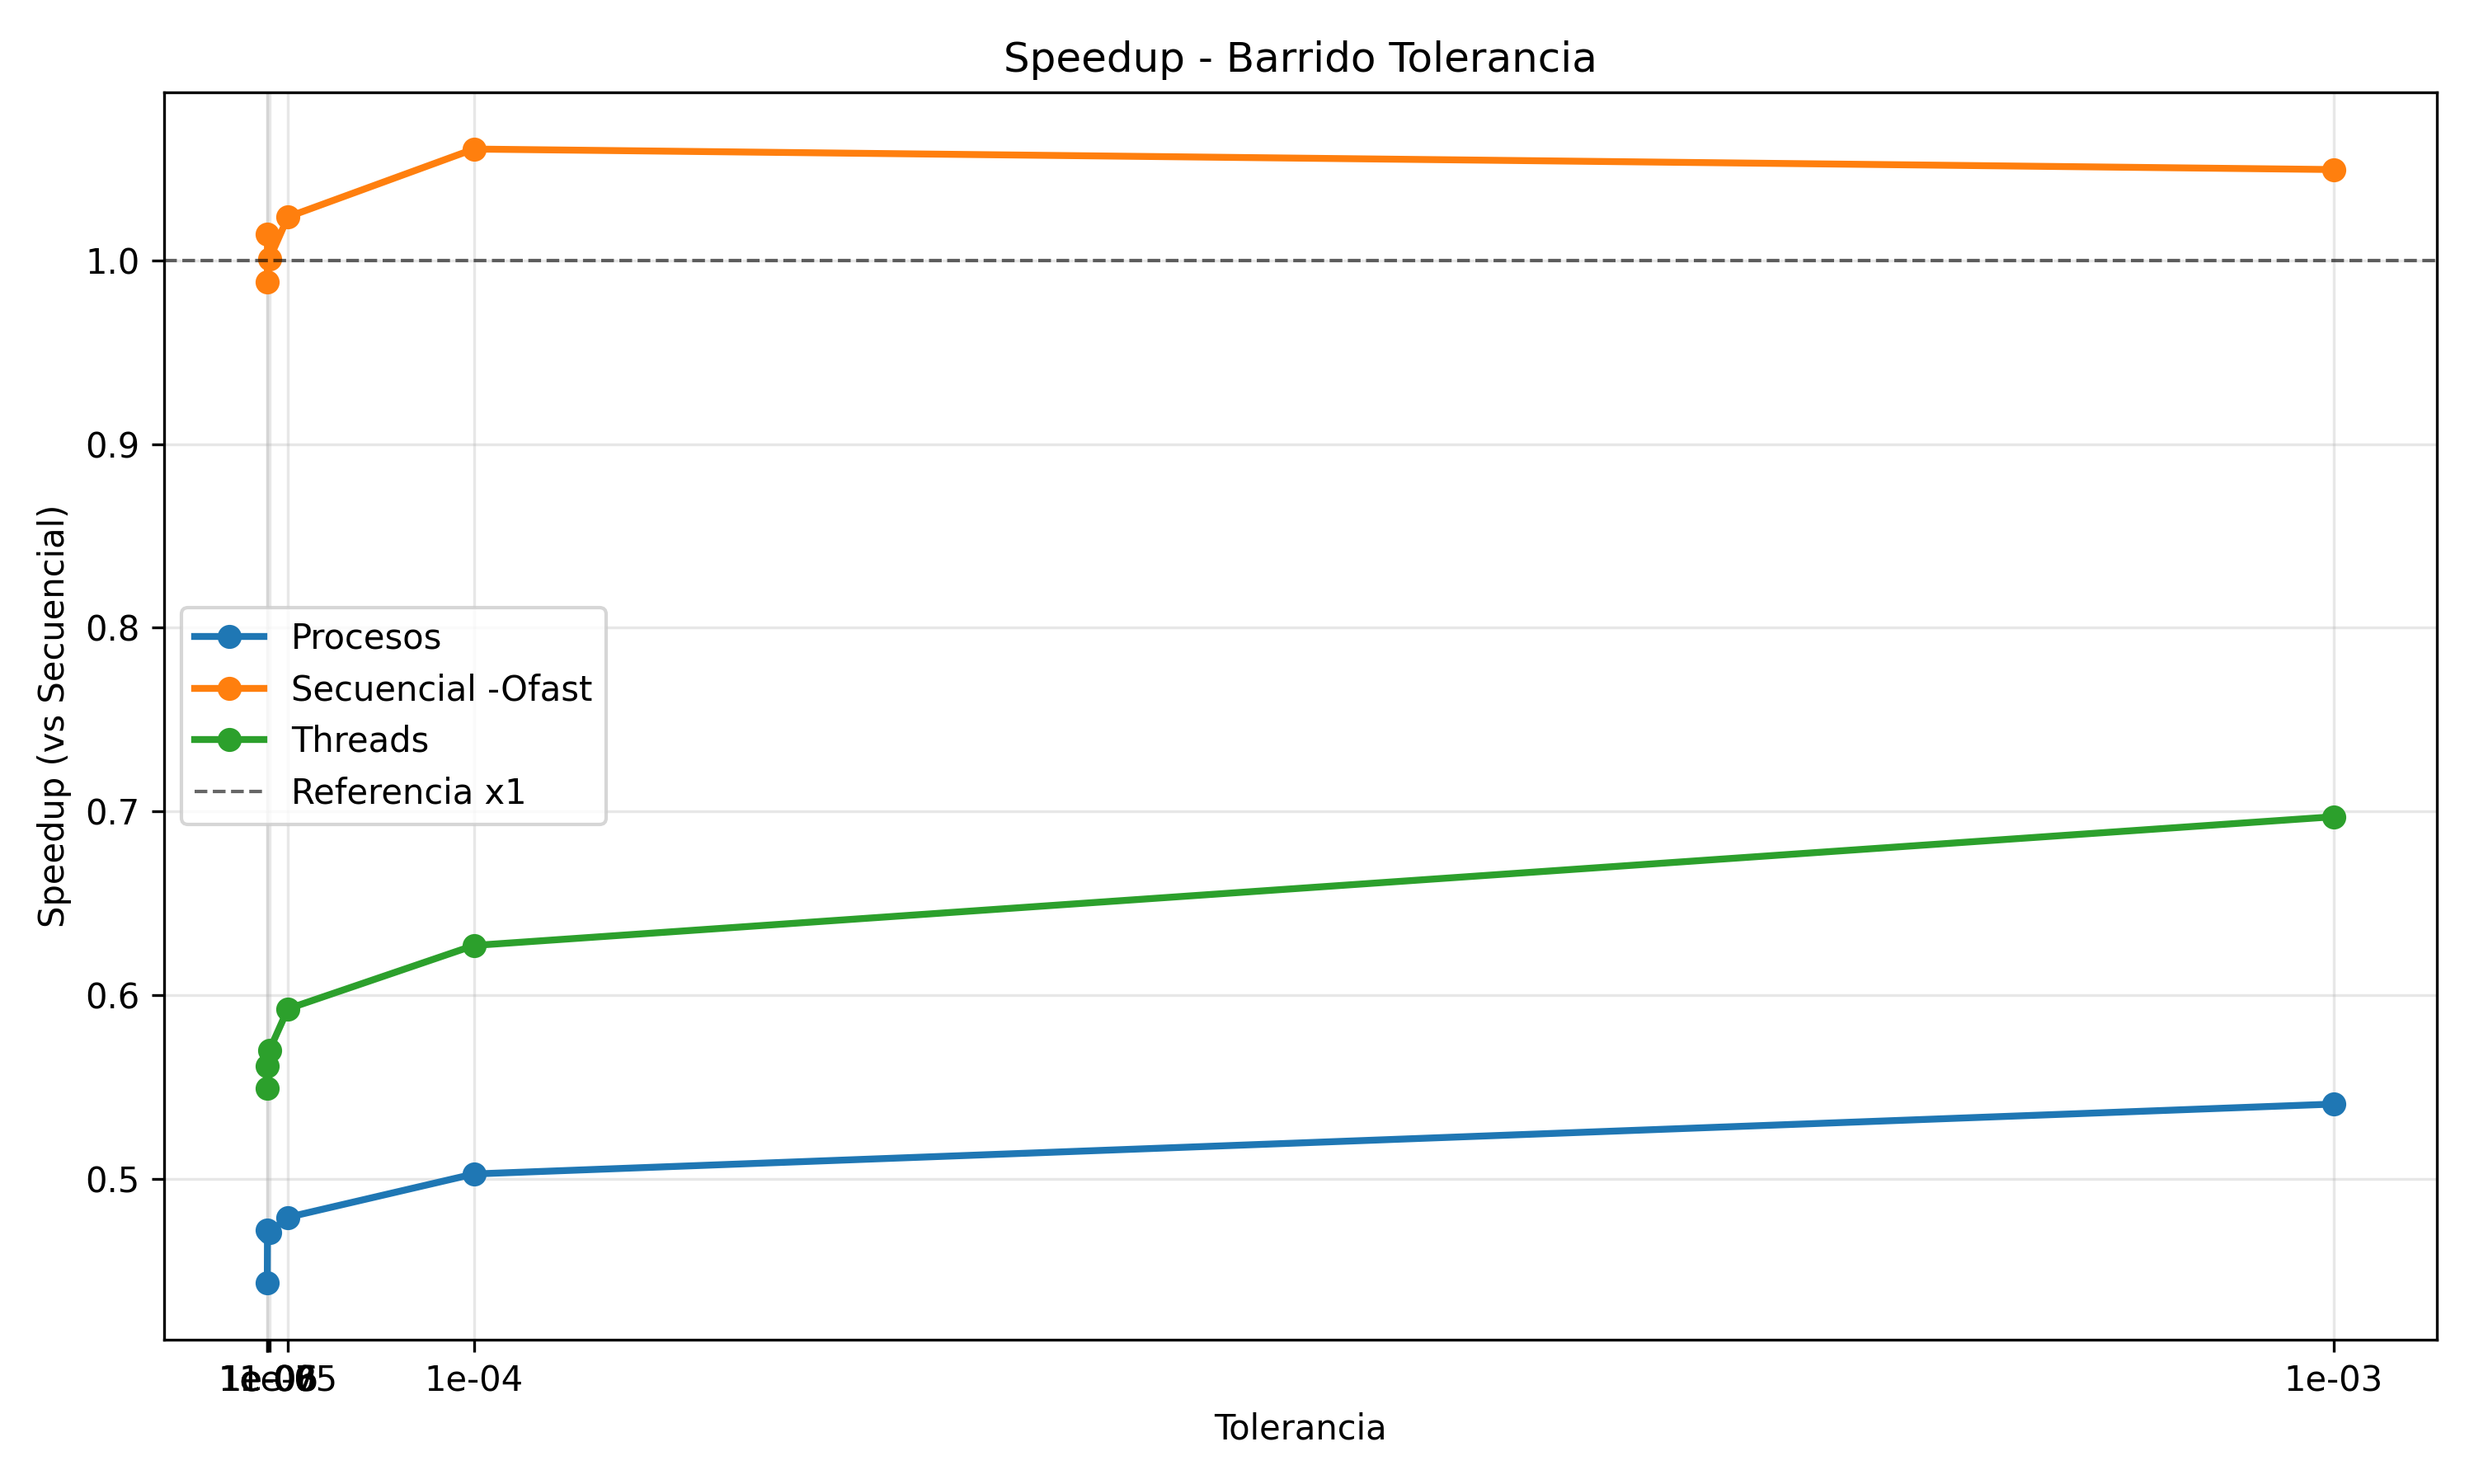
\includegraphics[width=0.85\textwidth]{plots/tol_sweep_speedup.png}
    \caption{Speedup (base secuencial) para barrido de tolerancia.}
\end{figure}

\section*{Resumen de hallazgos}

\begin{itemize}[leftmargin=1.2cm]
    \item Los hilos son la opción preferida para Jacobi por su baja latencia en memoria compartida.
    \item Conviene paralelizar solo en mallas grandes: para $K<10$, el paralelismo puede ser contraproducente.
    \item El cuello de botella principal en Jacobi es la barrera de sincronización obligatoria, que limita el \emph{speedup} máximo.
\end{itemize}

\end{document}
